%% Generates x) plot between 0 and pi
  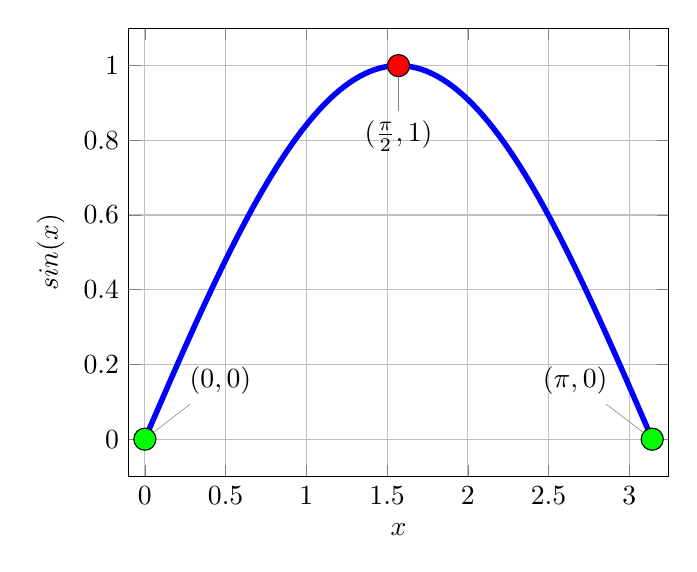
\begin{tikzpicture}
    \begin{axis}[ xlabel = $x$,
	  ylabel = {$sin(x)$},
	  ymin = -0.1, ymax = 1.1,
	  xmin = -0.1, xmax = pi + 0.1,
	  grid=both,
	  domain = 0:pi
	]
       \addplot[color=blue, line width=2pt, samples=100] 
          {sin(x*180/pi)} ;
       \addplot[only marks, mark options={fill=green,scale=2} ]
          coordinates { (0,0) (pi, 0) } ;
       \addplot[only marks, mark options={fill=red,scale=2} ]
	  coordinates { (pi/2, 1) };
	  
	  \node[pin=270:{$(\frac{\pi}{2}, 1)$}] at (axis cs:pi/2,1) {} ;
	  \node[pin=45:{$(0,0)$}] at (axis cs:0,0) {} ;
	  \node[pin=135:{$(\pi,0)$}] at (axis cs:pi,0) {} ;
    \end{axis}
  \end{tikzpicture}
